\subsection{Taggre : a task aggregator framework}
Our goal is to keep the natural way of describing parallelism in the linear solver.
%
Unfortunately, the granularity is too fine, it can takes up to 5 times longer to schedule a task than to do the computation inside this one.
%
To achieve this goal, we need to increase the granularity of the description of the problem.
%
Our idea is to create groups of tasks and schedule them at once in order to reduce the time lost in the overhead.
%
By this way, we will have less tasks which means that we can have less parallelism.


From starting with the finest representation of the parallelism under a DAG form, we need to a compute a new coarse-grained DAG with less tasks.
%
The principal difficulty is to keep the {\em Acyclic} property of the graph, a cycle introduce a dead lock in the graph scheduling (Fig.~\ref{fig:agg_invalid}).
%
The other difficulty is to maintain enough parallelism to be able to use all cores available.

\begin{figure}[!ht]
     \begin{center}
        \subfigure[Invalid aggregation]{%
          \label{fig:agg_invalid}
          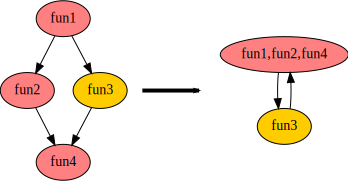
\includegraphics[width=0.4\textwidth]{agg_invalid}
        }%
        \hspace{0.15\textwidth}%
        \subfigure[Valid aggregation]{%
          \label{fig:agg_valid}
          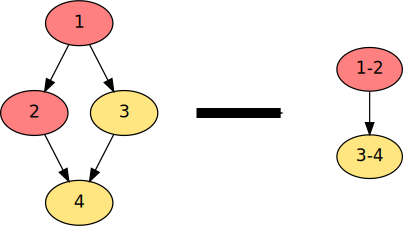
\includegraphics[width=0.4\textwidth]{agg_valid}
        }%
    \end{center}
    \caption{Example of two aggregations, the result of \ref{fig:agg_invalid} can't be schedule because of the cycle. The result of \ref{fig:agg_valid} can be schedule but there is no more parallelism.}
    \label{fig:agg_basic}
\end{figure}


We first developed a new programming interface based on Intel TBB that allow us to describe a complete DAG and schedule it with various scheduler (Fig~\ref{fig:runtime}).
%
With this interface, we can work on the DAG and make it coarser.
%
We called this interface Taggre, by using some heuristics, describe later in the thesis, a parallel program can continue to use its natural manner of describing parallelism and Taggre will do the effort of making it efficient (Fig.~\ref{fig:coarsening}).

%   (-_-)   %
\begin{figure}[t!]
  \centering
  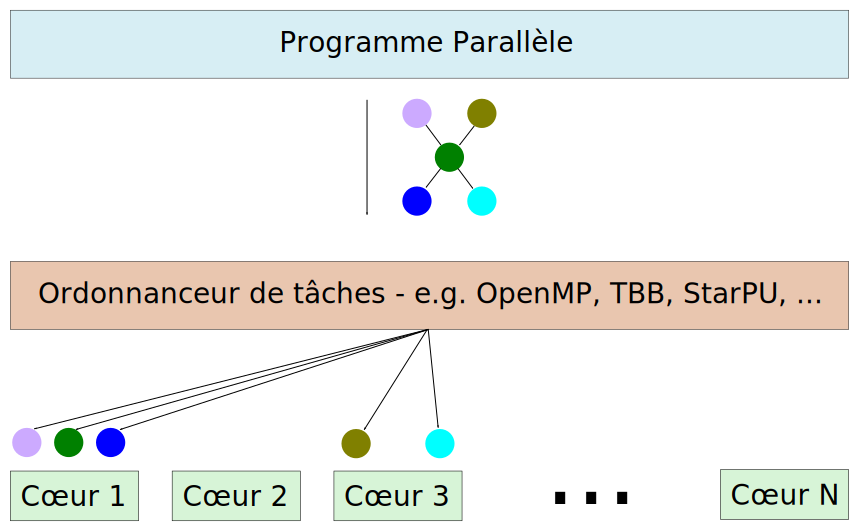
\includegraphics[width=0.8\textwidth]{runtime}
  \caption{}
  \label{fig:runtime}
\end{figure}

%   (-_-)   %
\begin{figure}[t!]
  \centering
  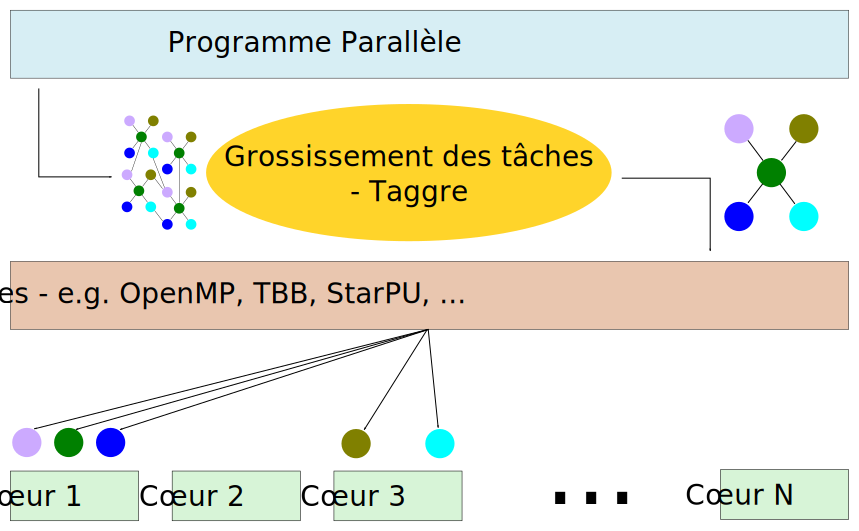
\includegraphics[width=0.8\textwidth]{coarsening}
  \caption{}
  \label{fig:coarsening}
\end{figure}
